%!TEX root = ../thesis.tex

\chapter{Results}
\label{ch:results}

\section{Exploring the Data: Cluster Analysis}

In order to better understand the player profiles, I used the $k$-means clustering
algorithm to separate player-seasons into clusters based on their tendencies. This
algorithm works by adjusting cluster centers in order to minimize inertia, also
known as within-cluster sum of squares:
$$
\sum_{i=1}^n \min_{c \in C} \lVert x_i - \mu_c \rVert^2
$$
where $C$ is the set of clusters and $\mu_c$ is the center of cluster $c$. The
$k$-means algorithm was chosen over other clustering algorithms for a few reasons;
first, it is a simple and easy-to-understand algorithm that often gives intuitive
results and has few parameters to tune other than the number of clusters. Second,
using inertia as the loss function for clustering assumes that clusters are convex
and isotropic, which is a reasonable assumption for player types; in other words,
the shapes of a cluster of players in player profile space should be roughly
spherical, rather than elongated.

In order to apply $k$-means to the player profiles, I used player profile data from
every season from 2006-07 to 2015-16, ignoring the ``replacement player'' category
used for the regression analysis so that the 360 players involved in the most plays
in each season were considered. As noted in section~\ref{sec:profiles}, the profiles
were normalized within each year by subtracting a given season's average for each
feature and dividing by its standard deviation; this is necessary because $k$-means
treats each datum as a point in space, so it is necessary for each feature to be on
the same scale.

Next, because $k$-means weights each dimension equally in computing distances, steps
must be taken to ensure that the many offensive features do not dominate the
relatively few defensive and rebounding features when distances are computed in
$k$-means. To remedy this problem, the variances of the five defensive and two
rebounding features were inflated by factors of 2 and 3 respectively so that they
are not drowned out by variance from the 25 offensive features. While these
adjustments were ad-hoc, they yielded intuitive results; moreover, the fact that
defensive and rebounding features are correlated with some offensive features
ensures that some of this signal is encapsulated in the offensive features. For
example, both rebounding features were heavily correlated with the proportion of ap
layer's shots taken from within four feet of the basket, as was block rate;
similarly, steal rate is correlated with a player's field goal percentage on corner
three-point attempts.

In order to determine the optimal number of clusters $k$, the goodness of fit for
a given value of $k$ was determined by the average silhouette score over all data
points. The silhouette score for a data point $x_i$ assigned to cluster $c$ of $N_c$
points is given by
$$
\frac{b_i - a_i}{\max(a_i, b_i)}
$$
where $a_i$ is the average distance between $x_i$ and all other points in cluster
$c$ and $b_i$ is the smallest average distance between $x_i$ and the nearest cluster
to which $x_i$ does not belong:
$$
a_i = \frac{1}{N_c} \sum_{x_j \in c} \lVert x_i - x_j \rVert \qquad
b_i = \min_{c' \neq c} \frac{1}{N_{c'}} \sum_{x_j \in c'} \lVert x_i - x_j
\rVert
$$
Therefore, a silhouette score close to one indicates that the point is
well-clustered, whereas a score close to zero indicates that a point is near the
border between clusters. The average silhouette scores for various values of $k$ are
shown in figure~\ref{fig:sils}.

\begin{figure}
    \centering
    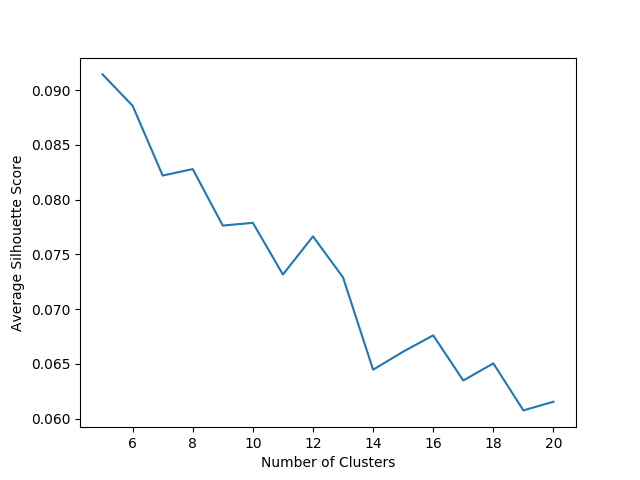
\includegraphics[width=0.75\textwidth]{figures/sil_scores}
    \caption{Average silhouette scores for various values of $k$.}
    \label{fig:sils}
\end{figure}

From this figure, we determine that the optimal number of clusters is $k=8$.  After
re-applying the $k$-means algorithm with $k=8$, we arrive at cluster means as shown
in figure~\ref{tab:clus_means}. Note that the means shown are the means of the data
that is after standardization by year but prior to inflating the variance of the
defense and rebounding features.

\begin{table}
    \centering
    \noindent\makebox[\textwidth]{%
    \begin{tabular}{cccc}
        pass
    \end{tabular}
    }
    \caption{TODO}
    \label{tab:clus_means}
\end{table}

\begin{figure}
    \centering
    \includegraphics[width=\textwidth]{figures/clus_means}
    \caption{Average silhouette scores for various values of $k$.}
    \label{fig:sils}
\end{figure}

TODO: interpret clustering, show means, exemplary players

\section{Cross-Validation Results}

As explained in section~\ref{sec:mod_sel}, cross-validation was done using three
randomly selected seasons on each run; many different cross-validation runs were
done in order to tune model hyperparameters; the results are summarized in
table~\ref{tab:cv_results}.

\begin{table}
    \centering
    \noindent\makebox[\textwidth]{%
    \begin{tabular}{cc|ccc}
        \toprule
        & Optimal Hyperparameters &
        Linear Regression & Random Forests & Gradient-Boosting \\[1em]
        Optimal Hyperparameters & & N/A & \parbox[c]{3cm}{300 estimators,\\ max
        depth 3} & \parbox[c]{3cm}{300 estimators,\\ max depth 3,\\ learning
        rate 0.1} \\ \midrule
        PCA & \parbox[c]{3cm}{5 components} & 1.263605* & 1.264270 &
        1.264506 \\ \midrule
        Isomap & \parbox[c]{3cm}{5 components,\\ 5 neighbors} & 1.266315 &
        1.266019 & 1.267266 \\ \midrule
        LLE & \parbox[c]{3cm}{5 components,\\ 5 neighbors} & 1.266406 & 1.266016 &
        1.267420 \\
        \bottomrule
    \end{tabular}
    }
    \caption{A summary of the results of hyperparameter tuning and
    cross-validation.}
    \label{tab:cv_results}
\end{table}

TODO: discuss

\section{Comparison to Baseline Model}

The motivation for this model is to incorporate play styles in order to improve upon
the regularized adjusted plus/minus model when predicting the relative performance
of two lineups. However, the RAPM framework proper is a method for evaluating
individual players and does not produce predictions for two arbitrary lineups;
therefore, an extension of the RAPM model is necessary in order to adapt it to
predict the outcome of a possession.  If one is to accept the RAPM model's
assumption that the outcome of a possession can be linearly allocated to the ten
players on the court as in~\eqref{eq:apm}, then a straightforward adaptation of the
RAPM model is to model the points per possession of one lineup against another as a
linear combination of the players' RAPM ratings with a home court adjustment:
\begin{equation} \label{eqn:baseline}
    y_i = \sum_{p \in OP_i} x_{\text{off}, p} - \sum_{p \in DP_i} x_{\text{def}, p}
    + \beta_{\text{HCA}}x_{\text{HmOff},i} + \beta_{\text{const}} + \epsilon_i
\end{equation}
where $y_i$ represents points on a possession $i$, $OP_i$ and $DP_i$ are the sets of
offensive and defensive players on the court for possession $i$ respectively,
$x_{\text{off}, p}$ and $x_{\text{def}, p}$ are player $p$'s computed ORAPM and
DRAPM ratings respectively, $x_{\text{HmOff}, i}$ is an indicator for whether the
home team is on offense for possession $i$, and $\epsilon_i$ is a
normally-distributed error term with zero mean. Then, the coefficients
$\beta_{\text{HCA}}$ and $\beta_{\text{const}}$ are optimized via ordinary least
squares. Note that the ORAPM and DRAPM values are not given coefficients; this is
because the RAPM model inherently assumes that these ratings combine linearly with
equal weights for each player. This assumption is made by the APM model
in~\eqref{eq:apm} wherein points on a possession is modeled as equal to the sum of
the offensive players' coefficients minus the sum of the defensive players'
coefficients, using an indicator to control for home court advantage and an
intercept term to control for league-wide average efficiency. In other words, this
is essentially the same prediction that a fitted RAPM model would make, were one to
use it to predict the outcome of a possession. Therefore, this model for predicting
points per possession follows logically from the RAPM framework for player
evaluation.

TODO: show coefficients, compare accuracy to full model

\section{Player Ratings}

Using the full model as specified in section~\ref{sec:mod_sel}, a given player $p$
can be evaluated by computing the expected point differential per possession that a
team of $p$ and four replacement players would achieve against a team of five
replacement players; this assigns a ``points above replacement'' rating based on how
much a player contributes to an otherwise replacement-level team. Expected point
differential per possession is computed by using the model to predict the expected
points per possession when the player's lineup is on defense and subtracting this
value from the predicted expected points per possession when the player's lineup is
on offense; for simplicity's sake, the offense is always assumed to be the home
team, so that the home court advantage cancels out during subtraction. Using the
model trained on data from the 2006-07 NBA season through the 2013-14 NBA season,
ratings were calculated for all (TODO: number?) players who played at least 820
minutes in the 2015-16 season, which corresponds to an average of 10 minutes per
game over the 82-game season; the best and worst of these ratings are shown in
table~\ref{TODO}. Recall that in computing these ratings, we use player profiles
built from data from both the prior season and the first half of the season in
question; therefore, the 2015-16 ratings are based partially on the 2015-16 season
itself and partially on the prior 2014-15 season. Moreover, remember that the
motivation of this model is to evaluate how the play styles of the members of a
lineup interact with each other, and having a low rating in table~\ref{TODO} simply
indicates that the player would not contribute well to a team of replacement-level
players against a team of replacement-level players. However, it is still possible
that the same player would be an effective contributor to different lineups or
against different lineups.

TODO: interpretation

\section{Lineup Ratings}

Just as players are evaluated by comparing them to replacement level, lineups can be
evaluated using the model by computing a lineup's expected point differential per
possession against a lineup of five replacement players. Each lineup that played at
least one possession in the 2015-16 season was evaluated, and the results are given
in table~\ref{TODO}.

TODO: interpretation

\section{Matchups Between Starting Lineups}

Another useful application of the model is that we can test how well we would expect
each team's starting lineup to perform offensively and defensively against every
other team's starting lineup. The expected points per possession for each possible
matchup is given in figure~\ref{TODO}, where the rows indicate the team on offense
and the columns indicate the team on defense; the values in the table represent the
how many points per 100 possessions the offensive lineup would be expected to score
against the defensive lineup \citep{Knuth1968}.

TODO: off-def matrix


TODO: diff matrix


TODO sections for:
starting lineup evaluation
trade evaluations
all star starters?
